\chapter{Structural Data: Formats, Databases, and Quality}
\label{ch:data-quality}

In October 1971, Walter Hamilton and his colleagues at Brookhaven National Laboratory
established the Protein Data Bank with seven structures~\cite{bernstein1977,berman2000}.\sidenote{The original seven
included myoglobin, hemoglobin, cytochrome~b5, alpha-chymotrypsin, lysozyme,
carboxypeptidase~A, and subtilisin BPN'.}
Hamilton and his colleagues reasoned that if crystallographers deposited their atomic coordinates
in a central archive, others could reuse them without repeating years of diffraction
experiments. Hamilton died just two years later, but the archive he founded grew
at a pace no one anticipated. By 1980 it held 75 structures. By 2000, roughly
13{,}000. As of early 2024, the Protein Data Bank contains over 210{,}000
experimentally determined macromolecular structures~\cite{burley2023}, and the AlphaFold Protein
Structure Database adds another 200 million predicted models on top of that~\cite{varadi2022,tunyasuvunakool2021}.

But quantity brought quality challenges that the founders could not have foreseen.
Early depositions often lacked the experimental data behind the coordinates. Some
structures were refined against insufficient data with too many free parameters.
Others contained errors in amino acid identity, stereochemistry, or chain
tracing that went undetected for years and then propagated silently through
hundreds of computational studies that treated PDB coordinates as ground truth.
Validation surveys have found stereochemistry and side-chain geometry errors in many
older archive entries~\cite{hooft1996}, and large-scale re-refinement benchmarks
show that modern protocols can improve both data fit and geometry for a majority
of deposited models~\cite{joosten2009}.
The situation improved with mandatory validation~\cite{gore2017}, but the lesson remains
relevant: every coordinate file carries assumptions, limitations, and potential
errors that a downstream user must understand.

This chapter covers the practical foundations of working with structural data.
We begin with the file formats used to encode atomic coordinates, move to the
databases that store and distribute them, and then spend the bulk of the chapter
on the validation metrics that distinguish a reliable structure from a
questionable one. We close with PDB-REDO, an automated re-refinement pipeline
that has improved thousands of older depositions using modern protocols~\cite{joosten2012actad,joosten2009}.


%% ========================================================================
\section{Coordinate formats}
\label{sec:coord-formats}

\newthought{A macromolecular structure} is, at bottom, a list of atoms with
three-dimensional coordinates. The file formats that encode this list have
shaped how the field thinks about structural data, and their quirks have
introduced persistent headaches.

\subsection{The PDB format}
\label{sec:pdb-format}

The original PDB format dates to the era of punch cards, with the modern
layout documented in historical and contemporary PDB archive
descriptions~\cite{bernstein1977,berman2000}. Each line is
exactly 80 characters wide, and each column has a fixed meaning. An
\texttt{ATOM} record, which describes a single atom in a standard residue,
packs the atom name, residue name, chain identifier, residue sequence number,
Cartesian coordinates $(x, y, z)$ in {\AA}ngstr\"oms, occupancy, and
temperature factor (B-factor) into those 80 columns:\sidenote{The
\texttt{HETATM} record uses the same column layout but denotes atoms in
non-standard residues such as ligands, metal ions, and modified amino acids.}

\begin{verbatim}
ATOM      1  N   ALA A   1      27.360  24.447   2.614  1.00 23.05
ATOM      2  CA  ALA A   1      26.426  25.514   2.229  1.00 19.82
ATOM      3  C   ALA A   1      26.996  26.920   2.307  1.00 17.56
\end{verbatim}

Columns 31--54 hold the $x$, $y$, and $z$ coordinates, each in a field
8.3 characters wide, giving a precision of 0.001~{\AA}. Columns 55--60 store
the occupancy (a number between 0 and 1), and columns 61--66 hold the
B-factor in {\AA}$^2$.

The format served the community for decades, but it was designed for small,
single-chain proteins. The chain identifier field is a single character,
limiting the format to 62 chains (A--Z, a--z, 0--9) in a single file. The
residue sequence number field is five digits wide, capping it at 99{,}999.
The atom serial number field allows at most 99{,}999 atoms. These limits
became untenable as structural biology moved toward large macromolecular
machines.\sidenote{The ribosome structure 4V9D, for instance, contains
over 400{,}000 atoms across more than 80 chains. It cannot be represented
in a single PDB-format file without workarounds.}

\subsection{The mmCIF format}
\label{sec:mmcif-format}

\newthought{The macromolecular Crystallographic Information File} (mmCIF)
replaced the PDB format as the master format of the Protein Data Bank in
2014 as part of the unified OneDep deposition system~\cite{young2017}.\sidenote{The PDB announced in 2014 that mmCIF would become the
standard archive format. PDB-format files are still distributed for
backward compatibility but are no longer generated for structures that
exceed PDB-format limits.}
Where the PDB format relies on column positions, mmCIF uses a
dictionary-based approach: each data item has a name drawn from a
controlled vocabulary, and values are associated with those names
explicitly. A fragment of mmCIF for the same atoms looks like this (see also the
mmCIF data dictionary~\cite{hall2005}):

\begin{verbatim}
loop_
_atom_site.group_PDB
_atom_site.id
_atom_site.type_symbol
_atom_site.label_atom_id
_atom_site.label_comp_id
_atom_site.label_asym_id
_atom_site.label_seq_id
_atom_site.Cartn_x
_atom_site.Cartn_y
_atom_site.Cartn_z
_atom_site.occupancy
_atom_site.B_iso_or_equiv
ATOM 1 N N ALA A 1 27.360 24.447 2.614 1.00 23.05
ATOM 2 C CA ALA A 1 26.426 25.514 2.229 1.00 19.82
ATOM 3 C C ALA A 1 26.996 26.920 2.307 1.00 17.56
\end{verbatim}

The format is more verbose, but it escapes all the column-width
limitations of the PDB format. Chain identifiers can be arbitrary
strings, atom counts are unbounded, and the dictionary enforces
a controlled vocabulary that makes automated parsing far less
error-prone. Equally important, mmCIF can encode metadata that
the PDB format simply cannot represent: details of multi-step
refinement protocols, experimental conditions, and links between
asymmetric-unit contents and biological assemblies.

\subsection{B-factors and occupancy}
\label{sec:bfactors}

\newthought{Two quantities in every coordinate file} deserve special
attention because they are frequently misunderstood.

The \emph{B-factor} (also called the temperature factor, displacement
parameter, or Debye--Waller factor) quantifies how much an atom's
position varies around its mean location. Under the assumption of
isotropic, harmonic displacement, the B-factor relates to the
mean-square displacement $\langle u^2 \rangle$ by
\begin{equation}
\label{eq:bfactor-isotropic}
  B = 8\pi^2 \langle u^2 \rangle.
\end{equation}
A B-factor of 20~{\AA}$^2$ corresponds to a root-mean-square
displacement of about 0.50~{\AA}, while a B-factor of 80~{\AA}$^2$
corresponds to roughly 1.01~{\AA}.\sidenote{Using \cref{eq:bfactor-isotropic}:
$\sqrt{\langle u^2 \rangle} = \sqrt{B / (8\pi^2)}$. For $B = 20$,
this gives $\sqrt{20/78.96} \approx 0.50$~{\AA}.}
The physical picture is that atoms in well-ordered regions of a
crystal (buried hydrophobic cores, for instance) have low
B-factors (often 10--20~{\AA}$^2$), while surface loops and
terminal residues can reach 60--100~{\AA}$^2$ or higher.

But B-factors are not purely physical. In crystallographic refinement,
the B-factor absorbs anything that smears electron density: genuine
thermal motion, static disorder across unit cells, partial occupancy
of a site, errors in the model, and even deficiencies in the data
(radiation damage, absorption effects, ice rings). A high B-factor
is a warning sign, not a diagnosis. It says ``this atom's position
is uncertain,'' without specifying why.

\newthought{Occupancy} records the fraction of unit cells in which
an atom actually occupies the modeled position. For most atoms in
a well-ordered crystal, the occupancy is 1.0. But if a side chain
adopts two distinct conformations (rotamer~A in 60\% of unit cells
and rotamer~B in 40\%), the crystallographer models both conformations
and assigns occupancies of 0.60 and 0.40 respectively. These are
recorded as ``alternate conformations'' (altlocs A and B in PDB
nomenclature).

Many software tools ignore alternate conformations by default, reading
only the first conformer or the one with the higher occupancy. This
is often acceptable for backbone analysis, but it can cause serious
errors in binding-site studies: a ligand interaction that depends on
a minor rotamer will be invisible if only the major conformer is read.
Careful users always check the occupancy column before trusting
coordinate-derived measurements.


%% ========================================================================
\section{Databases}
\label{sec:databases}

\newthought{The Protein Data Bank} is operated by the Worldwide Protein
Data Bank consortium (wwPDB), whose four member organizations each run a
regional portal: RCSB PDB in the United States, PDBe in Europe, PDBj in
Japan, and BMRB for NMR data.\sidenote{The wwPDB was formalized in 2003
to ensure a single, consistent archive regardless of where a structure
is deposited~\cite{wwpdb2003}. All four sites serve the same underlying data, but their
search interfaces, analysis tools, and API designs differ.}
Deposition is mandatory for structures reported in peer-reviewed
publications, and since 2008, experimental structure-factor amplitudes
(or NMR restraints, or cryo-EM maps) must be deposited alongside the
coordinates~\cite{wlodawer2008}. This policy was the single largest driver of improved
validation in the archive: without experimental data, independent
revalidation is impossible.

Each PDB entry is assigned a four-character accession code (e.g., 1CRN
for crambin, 6LU7 for the SARS-CoV-2 main protease). The entry
contains the atomic coordinates, metadata about the experiment
(resolution, space group, refinement software, data-collection
wavelength), and links to the deposited experimental data. Starting
in 2024, the PDB began transitioning to extended accession codes
to accommodate the growing archive.

\newthought{The Electron Microscopy Data Bank} (EMDB) stores
three-dimensional reconstructions from cryo-electron microscopy.
Unlike X-ray crystallography, where the deposited experimental
observables are structure-factor amplitudes, cryo-EM deposits
consist of density maps, three-dimensional grids of
electrostatic potential values. When an atomic model is built
into a cryo-EM map, the model goes to the PDB and the map goes
to the EMDB, cross-referenced by accession codes. The rapid
growth of cryo-EM since the ``resolution revolution'' of
2013--2014~\cite{kuhlbrandt2014}\sidenote{The development of direct electron detectors
and improved image-processing algorithms, recognized by the 2017
Nobel Prize in Chemistry to Dubochet, Frank, and Henderson,
pushed single-particle cryo-EM to near-atomic resolution for
the first time.}
has made EMDB one of the fastest-growing structural archives~\cite{lawson2011}.
As of 2024 it holds over 40{,}000 map entries.

\newthought{The AlphaFold Protein Structure Database,} launched in
2021 by DeepMind and the European Bioinformatics Institute~\cite{varadi2022}, represents
a different category of structural data entirely. Its entries are not
experimentally determined; they are predictions from the AlphaFold2
neural network~\cite{jumper2021}, trained on the PDB and co-evolutionary sequence data.
The database contains predicted structures for over 200~million
proteins, covering nearly every known protein sequence in UniProt.

This scale is staggering, but predicted structures carry their own set
of quality considerations. AlphaFold provides a per-residue confidence
metric called the predicted local distance difference test (pLDDT),
ranging from 0 to 100. Residues with pLDDT above 90 are generally
well-predicted; between 70 and 90, the backbone is usually reliable
but side-chain positions should be treated with caution; below 50,
the prediction is essentially unreliable and often corresponds to
disordered regions that lack a single defined structure in the first
place.\sidenote{The AlphaFold team explicitly warns against
interpreting low-pLDDT regions as structural~\cite{jumper2021}. These regions frequently
correspond to intrinsically disordered segments, linkers, and signal
peptides that are flexible in solution.}

The coexistence of experimental and predicted structural databases
creates a new challenge for the field. A researcher querying for a
protein's structure may find an AlphaFold prediction, a 2.5~{\AA}
crystal structure, and a 3.8~{\AA} cryo-EM map. Knowing how to
evaluate the reliability of each, and when to prefer one over
another, requires the validation framework we develop in the next
two sections.


%% ========================================================================
\section{Validation of crystallographic structures}
\label{sec:validation}

\newthought{Every crystallographic model} is the result of an
optimization procedure: the refinement program adjusts atomic
positions, B-factors, and sometimes occupancies to minimize the
disagreement between the diffraction pattern calculated from the
model and the diffraction pattern actually measured. Validation
asks whether the result of that optimization is physically
reasonable and supported by the experimental data, or whether the
refinement program has been given too much freedom and has
produced a model that fits the data by overfitting noise.

\subsection{Resolution}
\label{sec:resolution}

Before discussing agreement metrics, recall what resolution
means. In X-ray crystallography, resolution is the smallest interplanar
spacing $d_{\min}$ for which diffraction data were collected.
Higher-resolution data (smaller $d_{\min}$) contain more information about
atomic positions. At 3.0~{\AA} resolution, the overall fold and
secondary-structure elements are visible but individual atoms are not
resolved. At 2.0~{\AA}, most side chains can be placed confidently.
At 1.0~{\AA} or better, individual atoms are resolved and hydrogen
atoms begin to appear in the electron-density maps.\sidenote{Roughly
speaking, the number of independent observations in a diffraction
data set scales as $d_{\min}^{-3}$, so halving the resolution
increases the data-to-parameter ratio eightfold.}

Resolution is not a measure of model quality. It is a property of the
crystal and the diffraction experiment. A 2.0~{\AA} structure can be
poorly refined, and a 3.0~{\AA} structure can be carefully and
correctly built. But resolution sets a ceiling on the level of
detail that the data can support.

\subsection{The R-factor}
\label{sec:rfactor}

The oldest and most widely reported measure of model-data agreement is
the crystallographic R-factor:
\begin{equation}
\label{eq:rfactor-refinement}
  R = \frac{\displaystyle\sum_{hkl} \bigl|\, |F_{\mathrm{obs}}(hkl)| - |F_{\mathrm{calc}}(hkl)|\, \bigr|}
           {\displaystyle\sum_{hkl} |F_{\mathrm{obs}}(hkl)|},
\end{equation}
where $F_{\mathrm{obs}}$ and $F_{\mathrm{calc}}$ are the observed and
calculated structure-factor amplitudes and the sums run over all
measured reflections $(hkl)$.\sidenote{Structure factors are the Fourier
components of the electron density. Each reflection $(hkl)$ corresponds
to a specific spatial frequency, and its amplitude $|F(hkl)|$ and phase
$\phi(hkl)$ together determine the contribution of that frequency to
the map. Phases are lost in the diffraction experiment (the famous
``phase problem'') and must be recovered by experimental or
computational methods.}

An R-factor of 0.0 would mean perfect agreement between model and data.
A random arrangement of atoms gives an R-factor around 0.59. For a
well-refined protein structure at moderate resolution, R-factors
typically fall between 0.15 and 0.25.

The problem with $R$ as a sole quality indicator is that it always
decreases when you add more parameters to the model. Every additional
atom, every refined B-factor, every alternate conformation reduces $R$,
whether or not the added complexity is justified by the data. A
sufficiently parameterized model will fit noise as well as signal,
driving $R$ toward zero while producing a physically nonsensical
structure.

\subsection{R-free and overfitting}
\label{sec:rfree}

\newthought{Axel Br\"unger introduced $R_{\mathrm{free}}$} in 1992 to
address exactly this problem~\cite{brunger1992}.\sidenote{Br\"unger (1992), ``Free R value:
a novel statistical quantity for assessing the accuracy of crystal
structures.'' \textit{Nature}, 355, 472--475. The paper has been cited
over 15{,}000 times and changed standard practice in the field within
a few years of its publication.}
The idea borrows from cross-validation in statistics. Before refinement
begins, the crystallographer sets aside a randomly chosen subset of
reflections, typically 5\% of the total, as a ``test set.'' These
reflections are never used during refinement. $R_{\mathrm{free}}$ is
computed using \cref{eq:rfactor-refinement} but summed only over the test-set
reflections:
\begin{equation}
\label{eq:rfree}
  R_{\mathrm{free}} = \frac{\displaystyle\sum_{hkl \in \mathcal{T}}
    \bigl|\, |F_{\mathrm{obs}}(hkl)| - |F_{\mathrm{calc}}(hkl)|\, \bigr|}
           {\displaystyle\sum_{hkl \in \mathcal{T}} |F_{\mathrm{obs}}(hkl)|},
\end{equation}
where $\mathcal{T}$ is the test set. The complementary quantity,
$R_{\mathrm{work}}$, uses the remaining reflections (the ``working
set'').

If a refinement step genuinely improves the model, both $R_{\mathrm{work}}$
and $R_{\mathrm{free}}$ decrease. If the step overfits noise,
$R_{\mathrm{work}}$ decreases but $R_{\mathrm{free}}$ stays flat
or increases. The gap between $R_{\mathrm{work}}$ and
$R_{\mathrm{free}}$ is therefore a direct measure of overfitting.
For a well-refined structure, this gap is typically 2--5 percentage
points. A gap exceeding 7--8 points signals a problem.

The introduction of $R_{\mathrm{free}}$ had immediate practical
consequences. Several highly cited structures that had been refined
to suspiciously low R-factors were shown to have $R_{\mathrm{free}}$
values no better than random models, revealing that the low $R$ had
been achieved by fitting noise rather than capturing real structural
features. Deposition of $R_{\mathrm{free}}$ test-set flags became
standard practice, and journals began requiring both $R_{\mathrm{work}}$
and $R_{\mathrm{free}}$ in structure reports.

\subsection{Geometric validation}
\label{sec:geometric-validation}

\newthought{Agreement with the diffraction data is necessary but not
sufficient.} A model could fit the data well while containing bond
lengths, bond angles, or torsion angles that are physically impossible.
Geometric validation checks whether the model's internal geometry is
consistent with what we know from high-resolution small-molecule
crystallography and quantum-chemical calculations.

\begin{figure}
  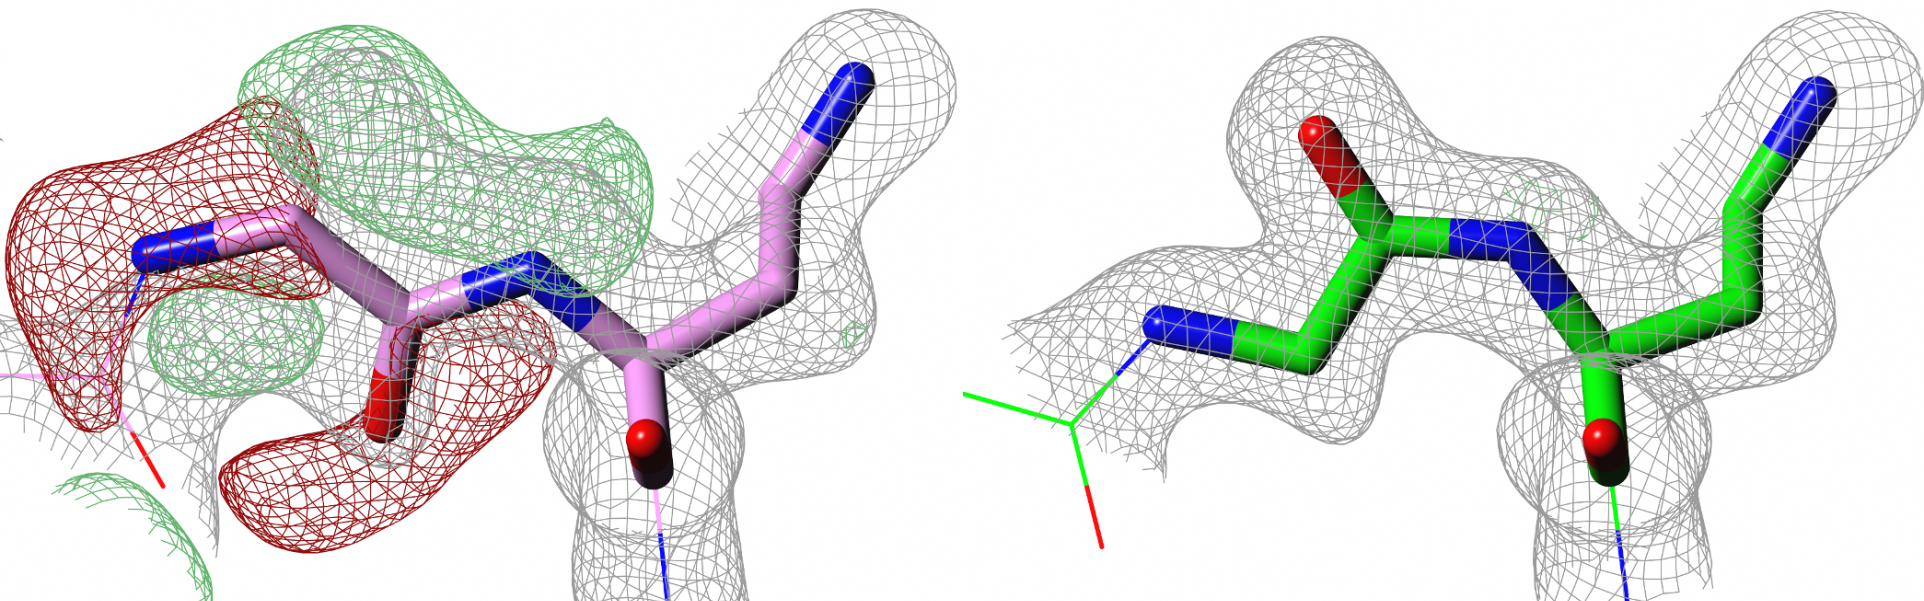
\includegraphics[width=\linewidth]{figures/ch02_electron_density.png}
  \caption{Electron density with difference maps: positive (green) and negative (red) peaks reveal model errors. Left: original; right: corrected.}
  \label{fig:electron-density}
\end{figure}

The most famous geometric check is the \emph{Ramachandran plot},
introduced by G.~N.~Ramachandran and colleagues in 1963~\cite{ramachandran1963}.\sidenote{%
Ramachandran, Ramakrishnan, and Sasisekharan (1963), ``Stereochemistry
of polypeptide chain configurations.'' \textit{J.\ Mol.\ Biol.}, 7,
95--99. The plot predates most of the structures it is now used to
validate.}
Each non-glycine, non-proline residue in a protein has two backbone
dihedral angles: $\phi$ (the torsion around the N--C$^\alpha$ bond)
and $\psi$ (the torsion around the C$^\alpha$--C bond). Steric
clashes between backbone atoms restrict the ($\phi$, $\psi$)
combinations that are physically accessible. Ramachandran and his
coworkers computed these allowed regions from hard-sphere
contact distances and found that most of the ($\phi$, $\psi$)
plane is sterically forbidden. Contemporary validation contours are typically
derived from high-resolution empirical distributions~\cite{lovell2003}.

\begin{figure*}
  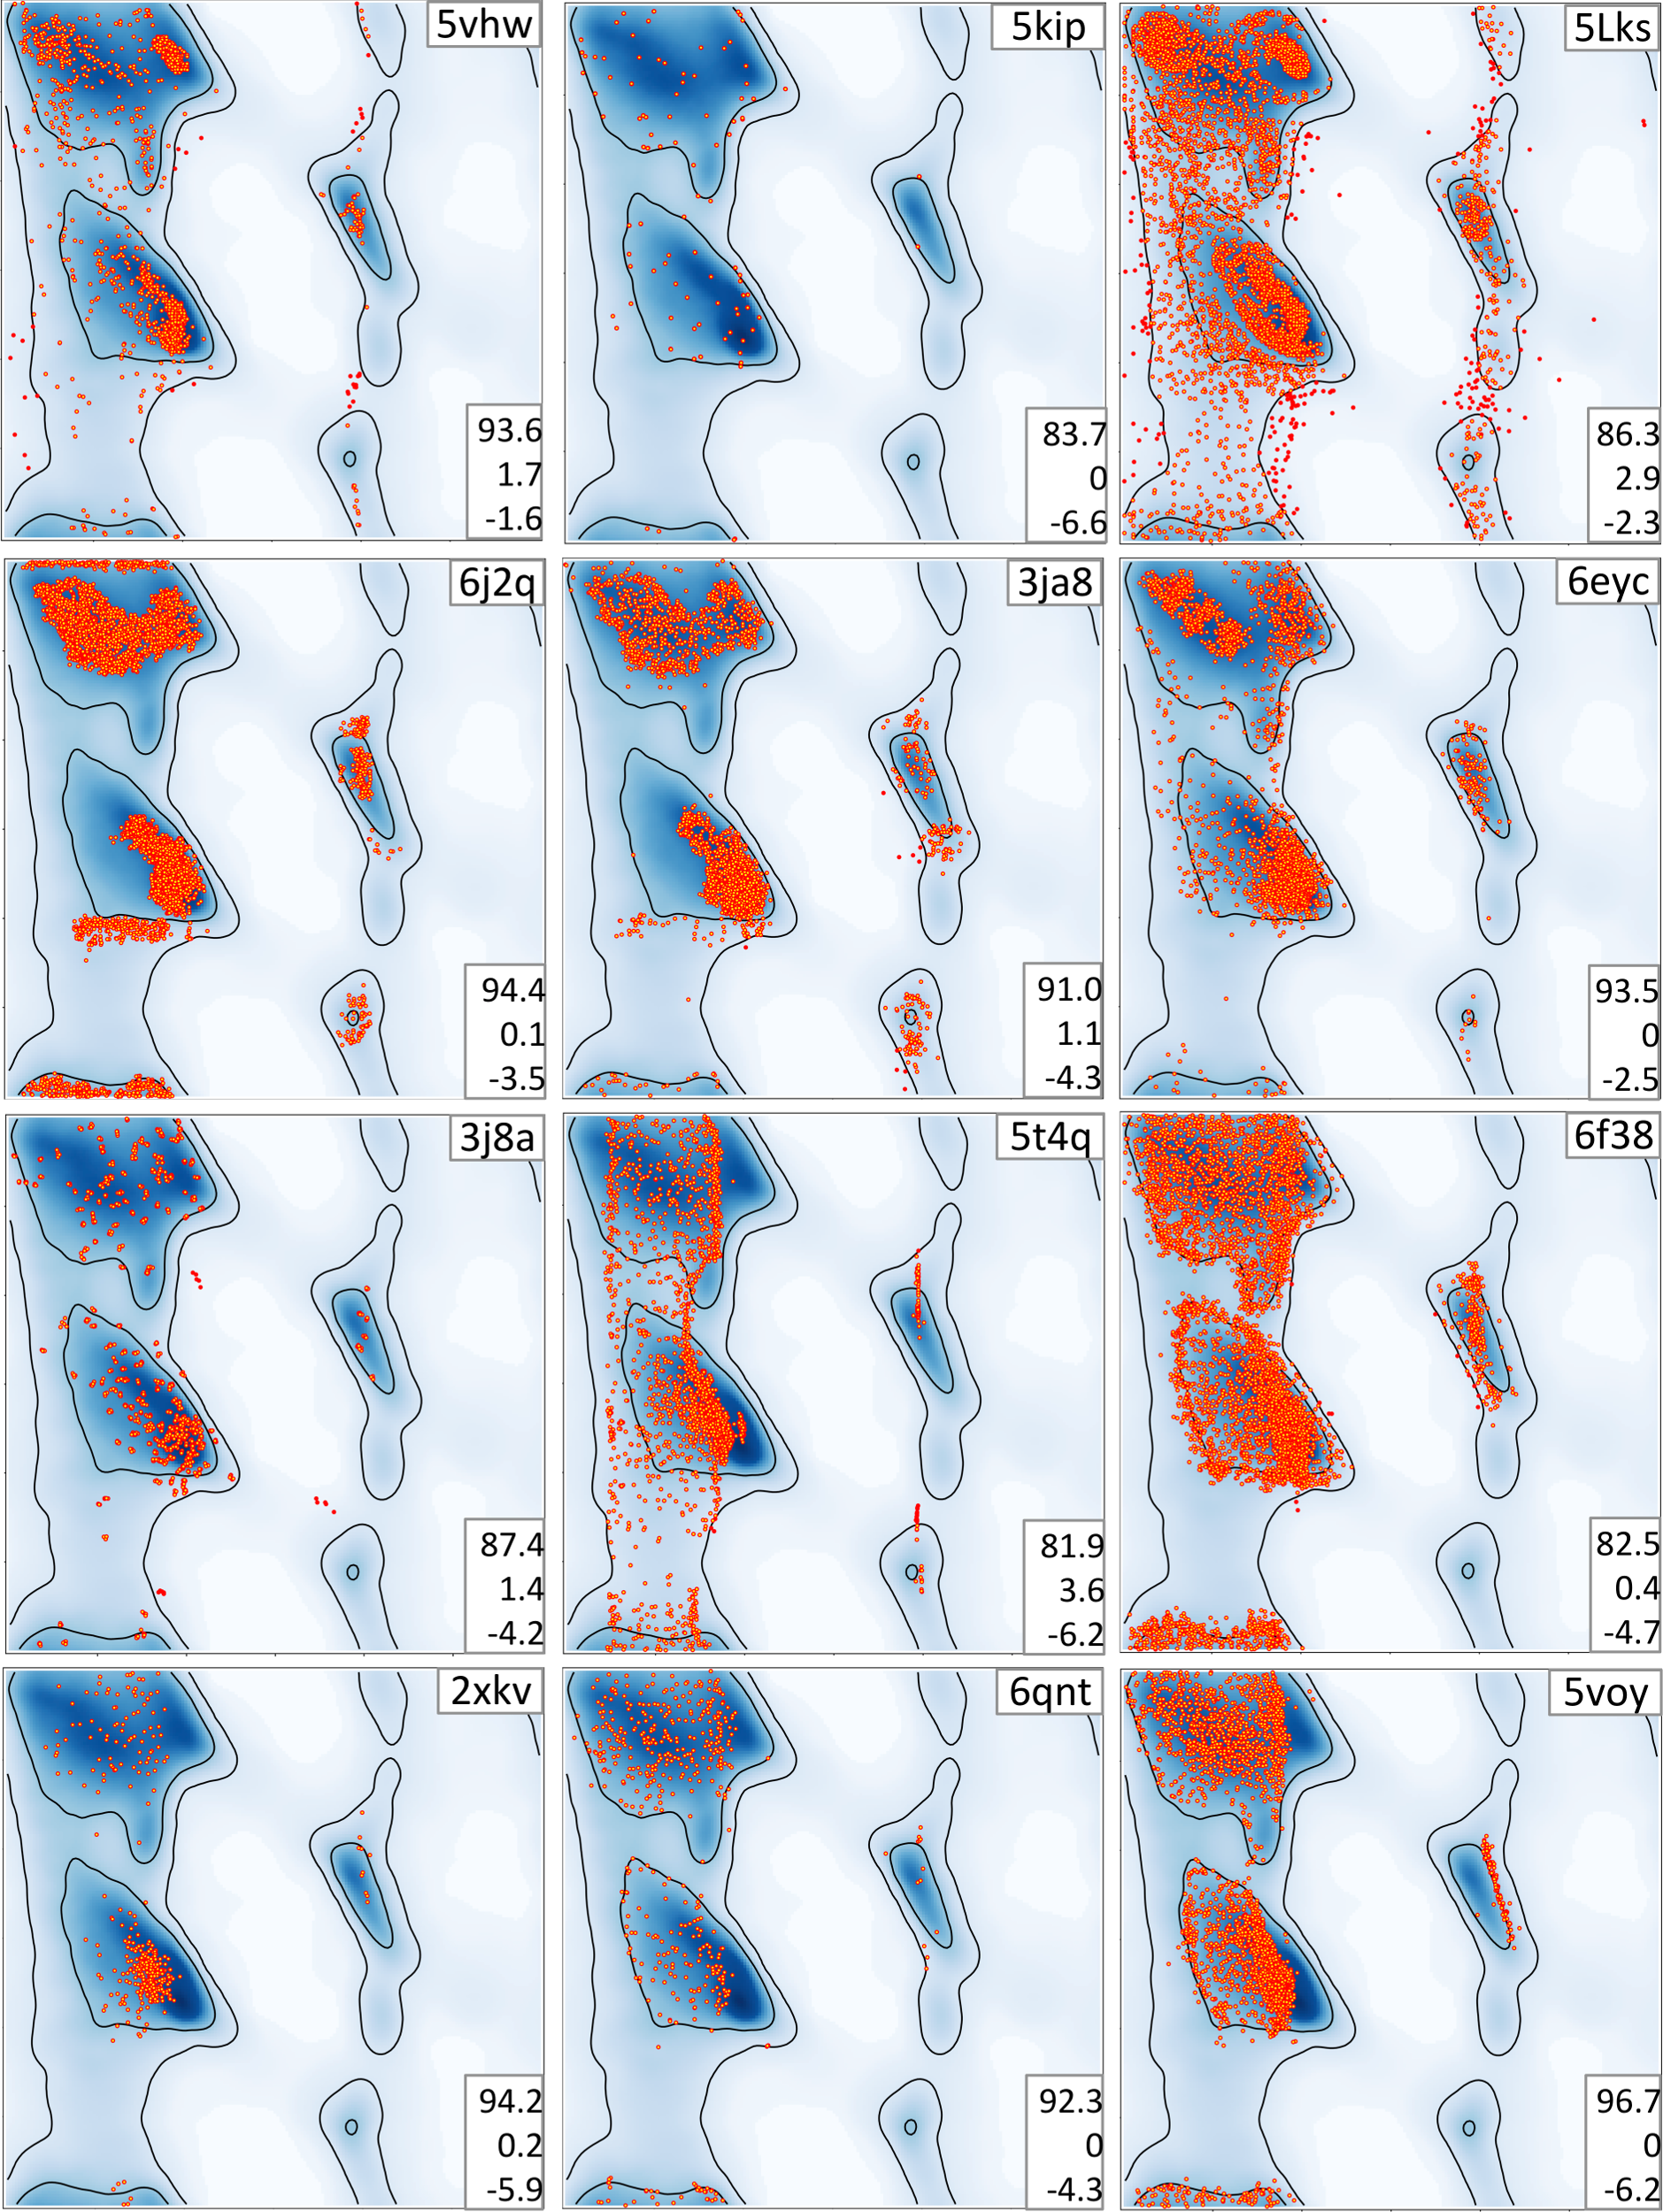
\includegraphics[width=\linewidth]{figures/ch02_ramachandran_validation.png}
  \caption{Ramachandran validation plots for twelve PDB structures. Red dots mark residue $(\phi,\psi)$ angles; contours show allowed regions. Percentages indicate favored-region occupancy.}
  \label{fig:ramachandran-validation}
\end{figure*}

When the plot is drawn using the observed $\phi$ and $\psi$ values
from a refined structure, the percentage of residues that fall outside
the allowed regions (the Ramachandran outlier percentage) is a
direct measure of model quality. A well-refined structure at
reasonable resolution should have fewer than 0.5\% outliers. An
outlier percentage above 2\% in a modern refinement is cause for
concern: either the structure contains genuine strain (rare, and
should be discussed in the publication) or the model is wrong at
those positions.\sidenote{Glycine, with no side chain, has a
much broader allowed region. Proline, constrained by its pyrrolidine
ring, is restricted to a narrow region near $\phi \approx -63°$.
Both are excluded from the standard outlier count and evaluated
separately.}

\subsection{MolProbity}
\label{sec:molprobity}

\begin{figure*}
  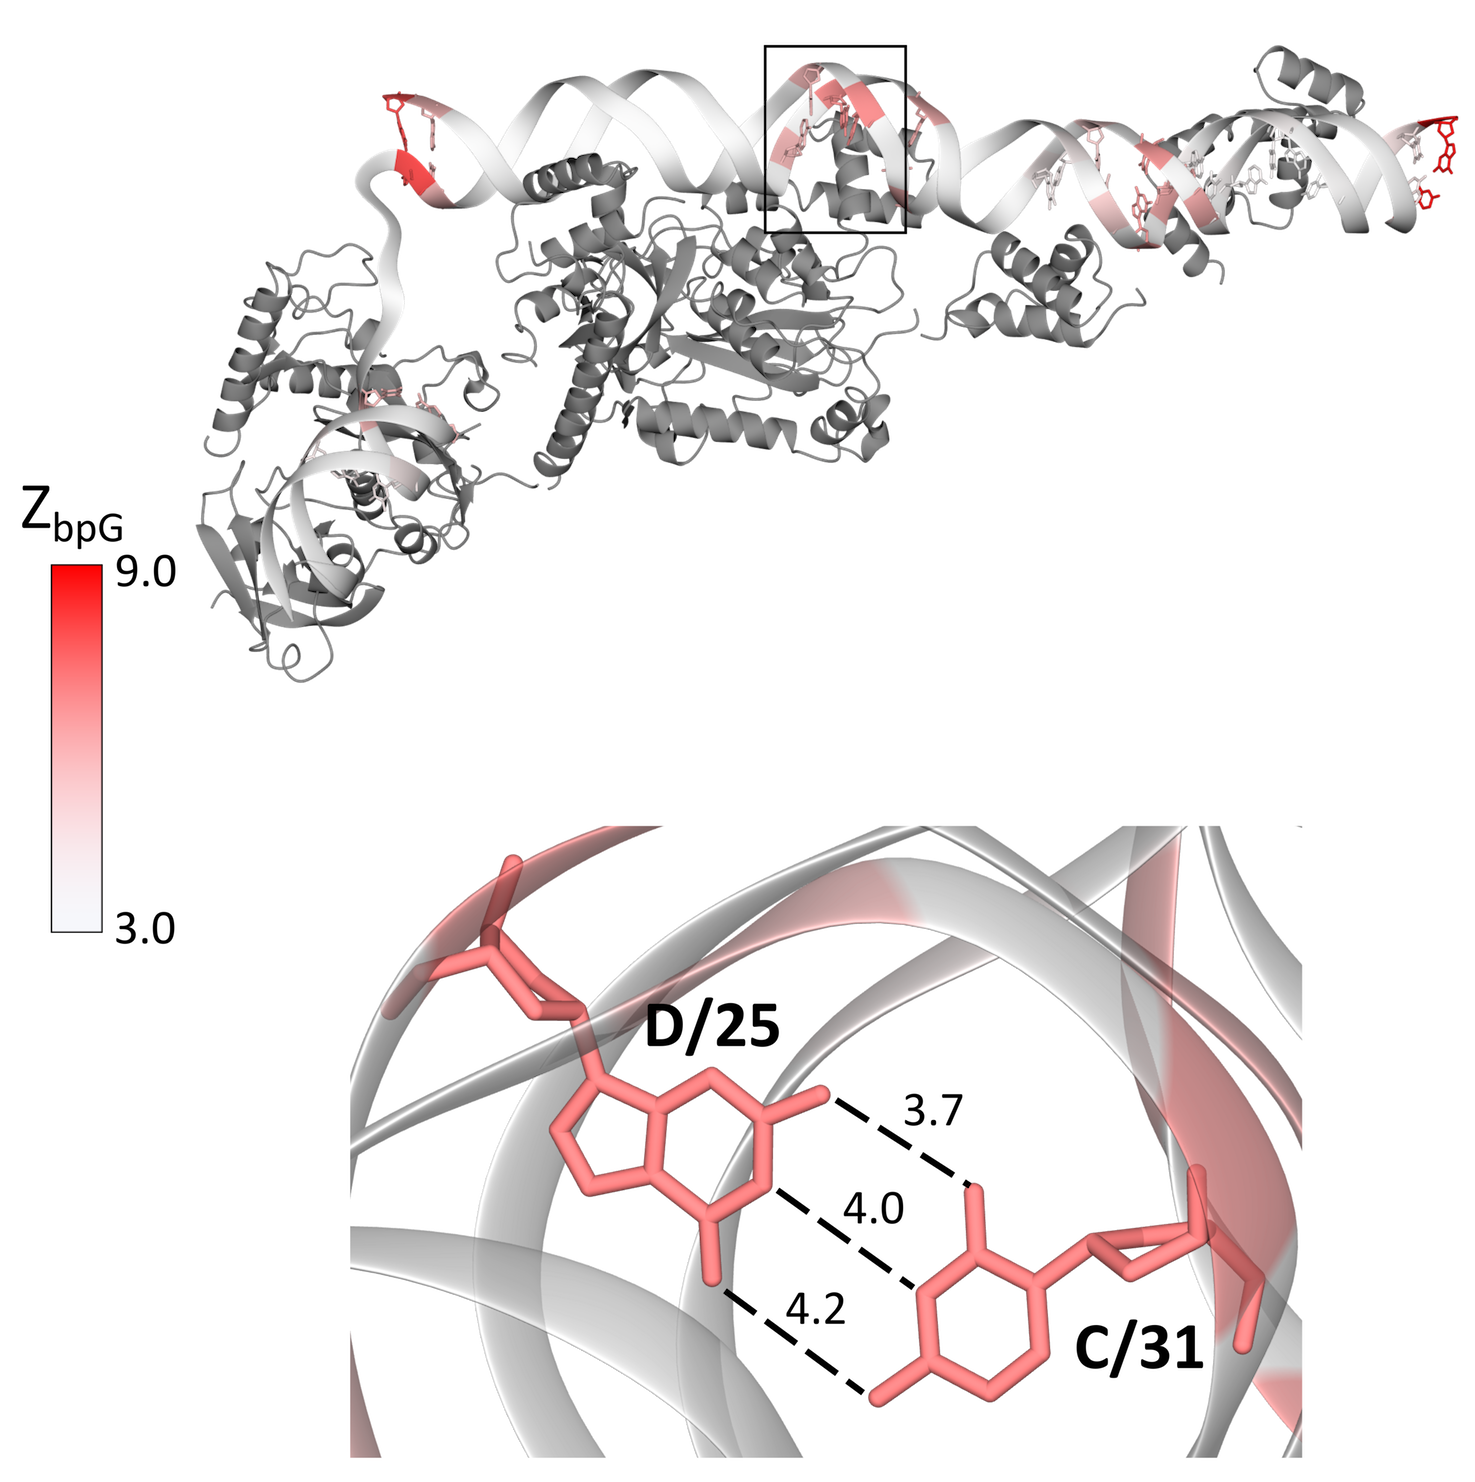
\includegraphics[width=\linewidth]{figures/ch02_validation_zscore.png}
  \caption{Structure validation by Z-score: residues with unusual geometry are highlighted in red on a DNA--protein complex. The inset shows a stacking geometry outlier detected at 3.7--4.2~\AA{} separation.}
  \label{fig:validation-zscore}
\end{figure*}

\newthought{MolProbity}, developed by the Richardson laboratory at
Duke University~\cite{chen2010,williams2018}, combines several geometric checks into a single
validation suite. Its key metrics include:

The \emph{clashscore}, defined as the number of serious steric
overlaps per 1{,}000 atoms, where a serious overlap is defined as
two non-bonded atoms whose van der Waals shells interpenetrate by
more than 0.4~{\AA}. After adding hydrogen atoms to the model (since
most crystal structures do not include them), MolProbity computes
all pairwise atomic distances and flags those that are too short. A
clashscore below 10 is considered good; below 5 is excellent. Older
structures refined without modern steric restraints sometimes have
clashscores above 40~\cite{word1999}.

\emph{Rotamer outliers} are side chains whose $\chi$ torsion angles
do not match any of the known preferred conformations (rotamers)
observed in high-quality structures. The rotamer libraries used by
MolProbity are derived from structures at 1.0~{\AA} resolution or
better, where the electron density is clear enough to determine
side-chain conformations unambiguously. A well-refined structure
should have fewer than 1\% rotamer outliers.

\emph{C$\beta$ deviations} flag residues where the position of the
C$\beta$ atom deviates from its ideal position (calculated from the
backbone geometry) by more than 0.25~{\AA}. A large C$\beta$ deviation
usually indicates an error in backbone or side-chain placement, or
occasionally a genuine backbone distortion.

MolProbity rolls these metrics into a single numerical score calibrated
against PDB-wide percentiles, making it easy to see at a glance whether
a structure's geometry is better or worse than average for its resolution
range. Journals now routinely require a MolProbity validation report as
part of the structure deposition process.

\subsection{Real-space correlation}
\label{sec:rscc}

\newthought{Global metrics like $R_{\mathrm{free}}$} tell you about the
model as a whole, but they cannot identify which parts of the model are
well-determined and which are not. A structure with $R_{\mathrm{free}}$
of 0.22 might have 90\% of its residues modeled correctly and 10\%
that are essentially guesses fitted into weak or ambiguous density. For
many applications (drug design, mutation analysis, molecular
dynamics), it is the local reliability that matters.

The \emph{real-space correlation coefficient} (RSCC) addresses this
need. For each residue (or ligand, or other model fragment), RSCC
measures the correlation between two electron-density values: the
density calculated from the full model and the density observed from
the experimental data.\sidenote{More precisely, RSCC is computed
over the grid points in the vicinity of the residue, comparing the
$2F_{\mathrm{obs}} - F_{\mathrm{calc}}$ map (which shows the
experimentally supported density) with the $F_{\mathrm{calc}}$ map
(which shows what the model predicts).}
It ranges from $-1$ to $+1$, with values above 0.9 indicating excellent
agreement and values below 0.7 indicating poor agreement. An RSCC below
0.7 for a residue in a 2.0~{\AA} structure is a strong signal that the
modeled conformation does not match what the crystal actually contains.

The wwPDB validation pipeline computes RSCC for every residue in every
deposited structure and includes the results in the validation report~\cite{gore2017}.
Users who plan to rely on a specific region of a structure (a binding
site, an active-site residue, a loop near a mutation site) should
check the RSCC values for those residues before drawing conclusions.


%% ========================================================================
\section{PDB-REDO: automated re-refinement}
\label{sec:pdb-redo}

\newthought{If validation metrics can identify problems,} the natural
next question is whether those problems can be fixed automatically.
The PDB-REDO project, developed by Robbie Joosten, Gert Vriend, and
colleagues at the Netherlands Cancer Institute and Radboud University,
answers this question with a qualified yes~\cite{joosten2012actad,joosten2009}.\sidenote{Joosten \textit{et al.}
(2012), ``PDB\_REDO: constructive validation, more than just looking for errors.''
\textit{Acta Cryst.} D\textbf{68}, 484--496.}

PDB-REDO takes an existing PDB entry (the deposited coordinates and
the deposited structure-factor data) and puts them through a modern,
fully automated refinement pipeline.

\begin{figure}
  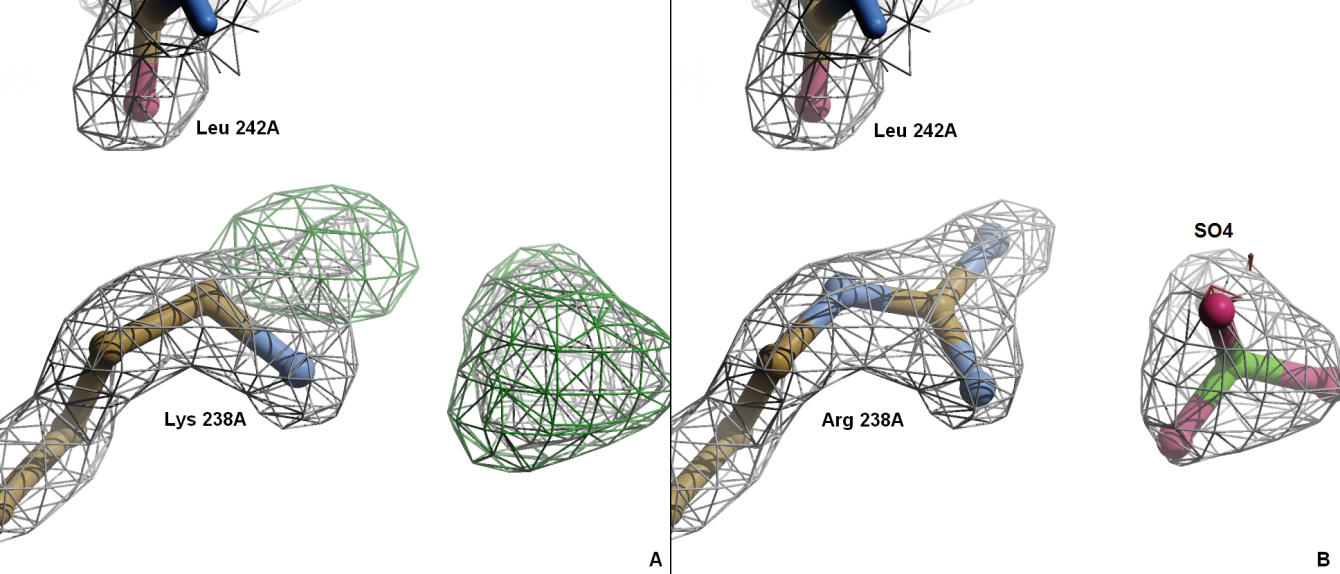
\includegraphics[width=\linewidth]{figures/ch02_pdbredo_correction.png}
  \caption{PDB-REDO in action: a Lys$\to$Arg correction with a sulfate ion placed into previously unmodeled density. (A)~Original model; (B)~re-refined model.}
  \label{fig:pdbredo-correction}
\end{figure} The pipeline uses the latest
version of REFMAC5 for maximum-likelihood refinement, applies
current geometric restraint libraries, rebuilds side chains where the
electron density supports different rotamers, adds or removes
alternate conformations, optimizes B-factor model complexity (deciding
whether each atom needs an isotropic B-factor, a TLS group
contribution, or both), and flips peptides and side chains where the
density is ambiguous.\sidenote{Peptide flips (180° rotations of the
peptide plane) and side-chain flips (e.g., swapping the N and O atoms
of asparagine or the N$\varepsilon$2 and O$\varepsilon$1 atoms of
glutamine) are common errors in crystal structures because these
atom pairs have similar electron density at moderate resolution.}

\newthought{The central tension in re-refinement} is between geometric
targets and electron-density fit. Geometric restraints penalize
deviations from ideal bond lengths, bond angles, and torsion angles.
Experimental data restraints penalize deviations between calculated
and observed structure factors. If the restraint weights are set
too heavily toward geometry, the model will have textbook-perfect
bond lengths but may not fit the density; set too heavily toward
data, and the model will follow every noise feature in the map at
the expense of physically reasonable geometry. PDB-REDO optimizes
this balance by systematically varying restraint weights and
selecting the combination that minimizes $R_{\mathrm{free}}$ while
keeping geometric outliers within acceptable ranges.

The results have been substantial. Across the PDB archive,
PDB-REDO improves $R_{\mathrm{free}}$ for roughly 75\% of the
structures it re-refines. Many structures from the 1990s and early
2000s, refined with software that is now two or three generations
old, show improvements of 5 percentage points or more in
$R_{\mathrm{free}}$, along with large reductions in Ramachandran
outliers and clashscores. A ligand modeled in a strained conformation
because the original refinement software lacked proper restraints can
be corrected. A loop built into weak density and left with B-factors
above 100~{\AA}$^2$ can sometimes be retraced into better density
that the original crystallographer missed.

\newthought{PDB-REDO also introduces a useful distinction} between
model completeness and model accuracy. A model is complete when it
accounts for every feature visible in the electron density: all
residues in the sequence, all ordered waters, all ligand atoms, all
alternate conformations. A model is accurate when the atoms that are
present are placed correctly. These goals can conflict. An
overzealous crystallographer might model residues into noise to achieve
completeness, producing an apparently full model with poor local
accuracy. Conversely, a cautious crystallographer might omit uncertain
residues, producing an incomplete but accurate model. PDB-REDO
attempts to optimize both simultaneously, removing atoms that are
not supported by density and refining the positions of those that
remain.

The practical lesson for users of structural data is that a PDB
entry is not the final word. It is a snapshot of the model as it
existed when the depositor finished working on it. That depositor
may have used outdated software, applied suboptimal restraint weights,
or simply run out of time. The PDB-REDO entry for the same structure
often represents a better model of the same experimental data, and
any serious downstream analysis should at least check whether a
PDB-REDO version exists.


%% ========================================================================
\section{A practical validation checklist}
\label{sec:checklist}

\newthought{The metrics described above} can be overwhelming in
isolation. In practice, evaluating a crystal structure for downstream
use requires checking several quantities together and interpreting
them in the context of the resolution and the specific region of
interest.

The resolution sets expectations. At 1.5~{\AA}, one should expect
$R_{\mathrm{free}}$ below 0.22, fewer than 0.2\% Ramachandran outliers,
and a clashscore below 5. At 3.0~{\AA}, $R_{\mathrm{free}}$ around
0.28 is typical, a few percent Ramachandran outliers may be tolerable
if they are in poorly ordered loops, and clashscores will be higher
because hydrogen atoms are less well-positioned. The wwPDB validation
report, available for every entry, shows how each metric compares to
other structures at the same resolution. This percentile-based
comparison is often more informative than the raw numbers~\cite{gore2017}.

For local quality, the RSCC and B-factor profiles should be examined
for the region of interest. A binding-site residue with RSCC above
0.9 and B-factors comparable to the surrounding protein is
well-determined. The same residue with RSCC below 0.7 and B-factors
twice the average should be treated as tentative. When alternate
conformations are present, the relative occupancies of each conformer
matter: a minor conformer at 15\% occupancy in a 2.5~{\AA} structure
is barely constrained by the data and should not be over-interpreted.

For structures from the AlphaFold database, the pLDDT score replaces
crystallographic metrics. Residues with pLDDT above 90 are generally
comparable in accuracy to experimental structures at 1.5--2.0~{\AA}
resolution~\cite{senior2020}.\sidenote{Comparison between AlphaFold predictions and
experimental structures in CASP14 showed that residues with pLDDT
$> 90$ had a median C$\alpha$ error of 0.6~{\AA}, comparable to
coordinate uncertainty in typical crystal structures at moderate
resolution.}
Residues between 70 and 90 have reliable backbone geometry but
uncertain side-chain placement. Below 50, the predicted coordinates
carry little information.


%% ========================================================================
\section{Chapter notes}
\label{sec:ch02-notes}

The history of the PDB has been recounted by Helen Berman, its long-time
director, in several retrospectives; Berman \textit{et al.} (2000,
\textit{Nucleic Acids Research}) provides a good overview of the archive's
evolution. The original seven structures deposited in 1971 are documented in
the PDB's own historical records and in Hamilton's correspondence, archived
at Brookhaven.

The PDB format specification is described in the ``PDB File Format Contents
Guide,'' version 3.30 (2011), available from the wwPDB. The mmCIF format
and its underlying data dictionary are maintained by the International Union
of Crystallography and are documented in Hall and McMahon (2005,
\textit{International Tables for Crystallography}, Vol.~G). For a practical
guide to parsing both formats, the Biopython project's \texttt{Bio.PDB}
module (Hamelryck and Manderick, 2003) and the GEMMI library (Wojdyr, 2022)
are widely used.

B-factors and their physical interpretation are discussed in Willis and
Pryor, \textit{Thermal Vibrations in Crystallography} (Cambridge University
Press, 1975). The problem of B-factor interpretation in macromolecular
crystallography, including the conflation of thermal motion, static disorder,
model error, and data pathologies, is treated in Rupp (2010),
\textit{Biomolecular Crystallography} (Garland Science), Chapter~12.

Br\"unger's 1992 paper introducing $R_{\mathrm{free}}$ is essential reading.
The history of its adoption and resistance to it in some quarters is
recounted in the Proceedings of the CCP4 Study Weekend (1993). Tickle
\textit{et al.} (1998, \textit{Acta Crystallogr.\ D}) provide a careful
statistical analysis of $R$-factor expectations as a function of resolution
and data-to-parameter ratio.

The Ramachandran plot's original formulation assumed hard-sphere radii. Modern
versions use empirical distributions from high-resolution structures; the
updated allowed regions used by MolProbity are described in Lovell
\textit{et al.} (2003, \textit{Proteins}). MolProbity itself is described in
Williams \textit{et al.} (2018, \textit{Protein Science}). The clashscore
metric was introduced by Word \textit{et al.} (1999, \textit{J.\ Mol.\
Biol.}).

PDB-REDO is described in Joosten \textit{et al.} (2012, \textit{J.\ Appl.\
Crystallogr.}) and its databank of re-refined entries is available at
\texttt{https://pdb-redo.eu}. A large-scale analysis of how re-refinement
improves older structures is presented in Joosten \textit{et al.} (2009,
\textit{J.\ Appl.\ Crystallogr.}), which examines the PDB-wide impact of
optimizing restraint weights and B-factor parameterization.

The AlphaFold Protein Structure Database is described in Varadi
\textit{et al.} (2022, \textit{Nucleic Acids Research}). For guidance on
appropriate use of AlphaFold models, see the best-practices document
maintained by the AlphaFold team and the community discussion in
Terwilliger \textit{et al.} (2024, \textit{Nature Methods}), which examines
when predicted structures complement or substitute for experimental ones.

For the reader interested in hands-on validation, the wwPDB validation
pipeline is described in Gore \textit{et al.} (2017, \textit{Structure}).
The validation reports it produces are available for every PDB entry on
the RCSB website and provide a concise, standardized summary of the metrics
discussed in this chapter.
